\chapter{System-Design und Implementierung}
\label{cha:systemdesign}

\section{Architektur}

\subsection{Von Anforderungen zum System-Design}
Den Anforderungen nach soll ein dezentrales Identitätsmanagementsystem entwickelt werden, dass die Möglichkeit bietet Credentials (wie z.B. Ausweisdokumente) auszustellen, zu überprüfen und selektiv zu veröffentlichen unter den - in Kapitel \ref{cha:anforderungsanalyse} genannten - Bedingungen. Daher werden zwei der drei Komponenten (Issuer, Verifier, Holder) implementiert. Der Issuer wird als CLI (Command-Line-Interface) implementiert und der Verifier als REST-API. Der Holder muss nicht implementiert werden werden, da die Plattformen jeweils Identity-Wallets anbieten. Als Use-Case wird die Erstellung eines Führerscheins illustriert. Dieser Führerschein (der Credential) wird von einer Autorität (Issuer) ausgestellt und kann von einem beliebigen Kontrolleur/Polizist/etc. (Verifier) überprüft werden.
Die in Kapitel \ref{cha:existierende Lösungen} angeführten Lösungen können alle diese Funktionen implementieren, daher wird anhand anderer Faktoren entschieden, welches Framework verwendet wird.

\subsection{Entscheidung über Framework}
Um sich für eine Architektur festzulegen, muss zunächst die Entscheidung über die darunterliegende Plattform getroffen werden. Dabei stehen die in Kapitel 5 betrachteten Lösungen zur Auswahl: Luniverse, Dock, PolygonId, Sovrin und Shocard. Für die Entwicklung des Prototypen wird PolygonID aus folgenden Gründen verwendet:
\begin{itemize}
	
	\item Polygon (als unterliegende Blockchain) zeigt folgende Vorteile auf \cite{ID54}:
	\begin{itemize}
		\item Die Blockchain skaliert hervorragend mit einer steigenden Anzahl von Transaktionen
		\item Geringe Transaktionskosten
		\item Hohe Interoperabilität mit Ethereum
		\item Etablierte Plattform und weite Verbreitung im Markt
	\end{itemize}
	
	\item PolygonId:
	\begin{itemize}
		\item Möglichkeit zum Widerruf von Informationen gegeben
		\item Informationen sind überprüfbar
		\item Selektive-Disclosure implementierbar
		\item kompatibel mit allen Anforderungen
		\item Unterstützt W3C Standard für VC's
		\item Credential Exchange erfolgt nach Identity-Foundation Standard
	\end{itemize}
\end{itemize}
\subsection{Grobe Architektur}
Prinzipiell besteht die Architektur aus drei Komponenten: Einem Verifier, einem Issuer und dem Holder. Jede dieser drei Komponenten laufen unabhängig voneinander und können mit fremd-implementierten Instanzen kommunizieren. Das hier dargestellte Szenario ist das Erstellen, Übertragen und Verifizieren von einem digitalen Führerschein auf der Blockchain. Die System-Architektur kann in der Grafik \ref{fig:design} betrachtet werden.
\begin{figure}[H]
	\centering
	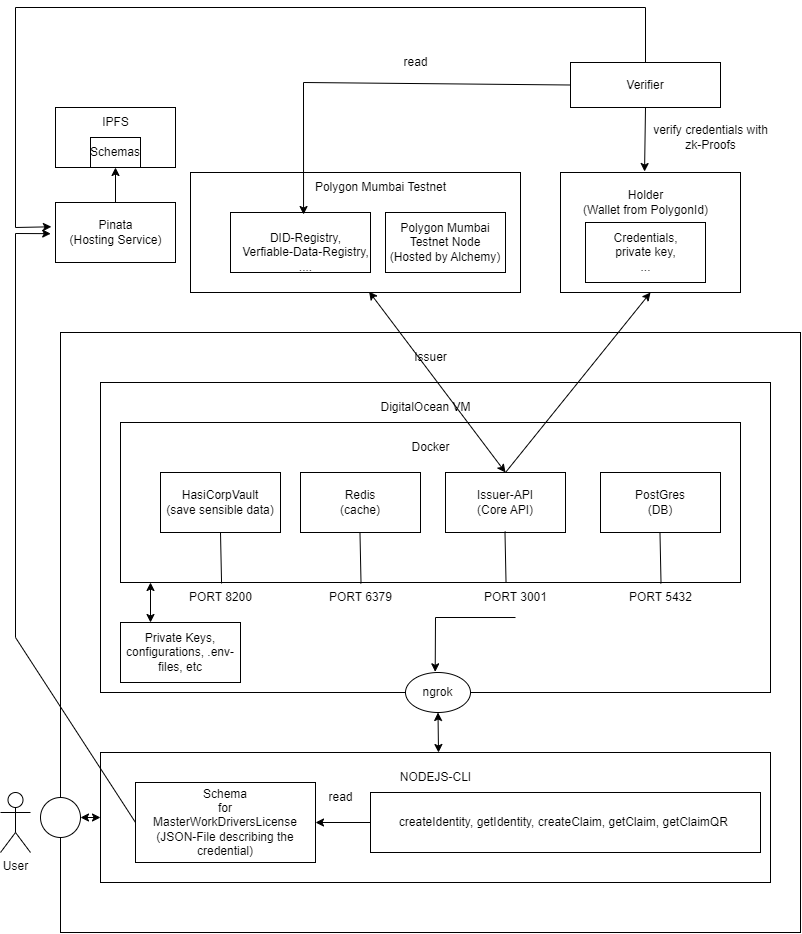
\includegraphics[scale=0.5]{media/system-design}
	\caption{System-Design des Prototyps}
	\label{fig:design}
\end{figure}
Es ist zu erkennen, dass der Issuer die zentrale Komponente ist. Um den Issuer zu hosten wird eine virtuelle Maschine von DigitalOcean \footnote{https://www.digitalocean.com/} verwendet. VMs werden bei DigitalOcean auch Droplets genannt.

Auf dem Droplet läuft eine Docker-Instanz, die alle in der Grafik darstellen Komponenten orchestriert. Das einzige Image, das auch von extern erreichbar sein muss ist das 'issuer-api'-Image, da dieses die REST-API Anfragen erhält. Für Letzteres wird 'ngrok' \footnote{https://ngrok.com/} verwendet. Ngrok hat die Funktion die lokale IP-Addresse (127.0.0.1) öffentlich durch einen Tunnel zugänglich zu machen. Dieser Tunnel wird vom NodeJs-Cli verwendet, um Anfragen über die API an den - von Alchemy \footnote{https://www.alchemy.com/} gehosteten - Netzwerk-Knoten weiterzuleiten. Alchemy wird benötigt, da mit Knoten des Polygon-Netzwerks kommuniziert werden muss und Alchemy diese zur Verfügung stellt. Die Schemas müssen öffentlich zugänglich sein, da sie unter anderem im Verifier und Issuer referenziert werden. Um dem ursprünglichen Gedanken der Dezentralität treu zu bleiben werden auch die Schemas dezentral - über IPFS \footnote{https://ipfs.tech/} - gespeichert. Als Schnittstelle zwischen IPFS und der Anwendung wird Pinata \footnote{https://www.pinata.cloud/} verwendet. IPFS ist eine Platform, die dem dezentralen Speichern von Inhalten dient und Pinata hostet IPFS-Knoten, damit diese nicht lokal aufgesetzt werden müssen. Das dort gehostete Schema ist in Grafik \ref{schema} illustriert.
\begin{lstlisting}[language=json,firstnumber=1, caption=Schema des Credentials, label=schema]	
		[...]
		"MasterWorkDriversLicense": {
			"@context": {
			 [...]
				"TypeOfVehicle": {
					"@id": "polygon-vocab:TypeOfVehicle",
					"@type": "xsd:string"
					[...]
					
					"enum": [
						"Car",
						"Truck",
						"Scooter",
						"Motorcycle"
					],
					
				},
				"YearOfReceipt": {
					"@id": "polygon-vocab:YearOfReceipt",
					"@type": "xsd:integer"
				}
			},
			[...]
		}
	}
	]
}
\end{lstlisting}
Es ist zu erkennen, dass der Führerschein für den Prototypen aus zwei Attributen besteht:
\begin{itemize}
	\item YearOfReceipt: Ein Integer, der das Jahr darstellt an dem der Holder den Führerschein erworben hat
	\item TypeOfVehicle: Ein String, der den Typ des Vehicle beschreibt. Hierbei gibt es vier Typen: 
	
	\begin{itemize}
		\item Car
		\item Truck
		\item Scooter
		\item Motorcycle
	\end{itemize}
\end{itemize}

Zum Erstellen der Schemata stellt PolygonId einen Schema-Builder zur Verfügung \footnote{https://schema-builder.polygonid.me/}. \\
Der Issuer stellt den Führerschein aus, indem er einen QR-Code erstellt, der die Informationen über den Credential enthält (also Typ und Jahr). Dieser QR-Code kann mit der PolygonID-App gescannt werden. Der Holder kann die Informationen über den Führerschein einsehen und akzeptieren. Im Anschluss befindet sich der Credential im Identity-Wallet. Details über diesen Prozess sind in den folgenden Kapitel beschrieben. Der nächste Schritt ist, dass ein Verifier einen Query definiert, der wie folgt aussehen könnte:
\begin{lstlisting}[language=json,firstnumber=1]
{[...]
	id: 1,
	circuitId: 'credentialAtomicQuerySigV2', // algorithmus zum Erstellen des zk-Proofs
	query: {
		allowedIssuers: ['*'],
		type: 'MasterWorkDriversLicense', // im Schema definierter Typ
		context: 'https://ipfs.io/ipfs/QmTSd6saivXHysRopQdM1yswp2qyFwobL7fwuFpkVTS8gd',
		credentialSubject: {
			YearOfReceipt: {
				$lt: 2022,
			},
		},
	},
	[...]
}
\end{lstlisting}
Der hier dargestellte Query überprüft primär, ob der Führerschein des Holders älter als vom Jahr 2022 ist. Indirekt fragt er ebenso ab, ob der Nutzer den beschriebenen Credential besitzt und ob dieser noch gültig ist. Ist dies der Fall, so wird der zk-Proof an den Verifier gesendet.
\newpage
\section{Kommunikation der Komponenten}
Die Kommunikation der Komponenten ist in Abbildung \ref{fig:komm} dargestellt.

\begin{figure}[H]
	\centering	
	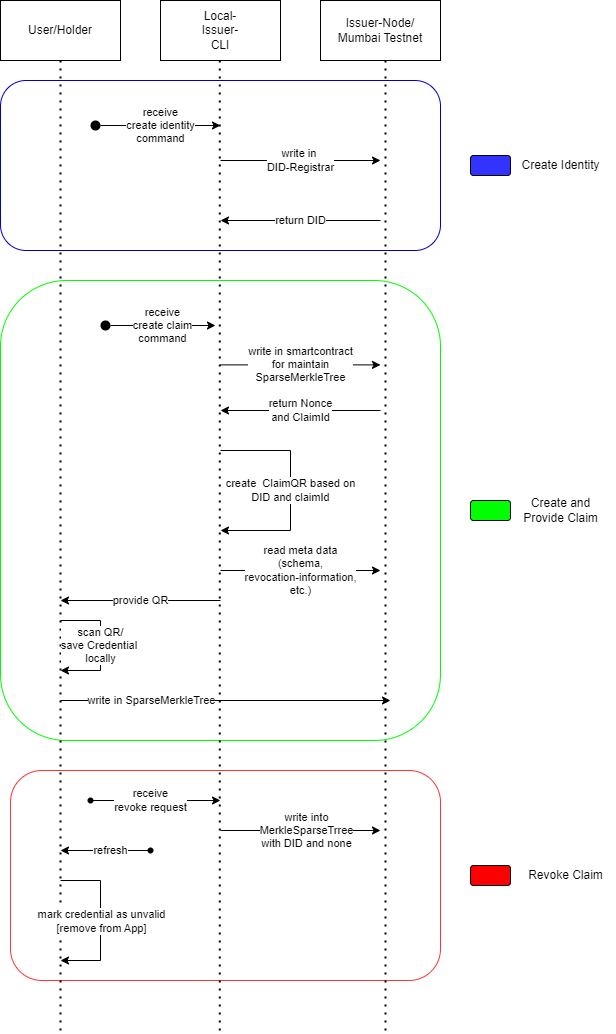
\includegraphics[scale=0.55]{media/ablaufdiagram.drawio}
	\caption{Kommunikationsdiagramm des Issuers, Holder und der Blockchain}
	\label{fig:komm}
\end{figure}
\newpage
Dabei sind jeweils die Prozesse zum Erstellen einer Identität, Erstellen und Zuweisen von Credentials und das Widerrufen von Credentials illustriert. Die drei Akteure sind jeweils der User/Holder (in diesem Falle die PolygonID-App), das Issuer-CLI (mit Node-JS implementiert) und der Issuer-Node (über DigitalOcean gehostet). Es ist zu erkennen, dass jede der drei Aktivitäten durch das CLI initialisiert wird. In der 'create Identity' Aktivität wird eine Identität erstellt, wobei in das DID-Registrar geschrieben wird. Diese Komponente ist dafür zuständig DID's und DID-Documents zu verwalten und befindet sich in der Blockchain.
Bei dem Erstellen und Zuweisen von Claims spielt die Blockchain insofern eine wichtige Rolle, als dass in den 'Sparse-Merkle-Tree' geschrieben wird (siehe \ref{merkle}). Auch auf das Widerrufen von Credentials trifft dies zu.
\section{Der Issuer}
Der Issuer kann im Polygon-Framework auf zwei Weisen realisiert werden:
\begin{itemize}
	\item 'On-Chain': Das Ausgabe der Credentials geschieht hierbei 'on-chain', also innerhalb der Blockchain. Implementiert wird die Logik mittels Smart-Contracts, was bedeutet, dass die Logik beliebig erweitert werden kann. Die anzuwendende Programmiersprache ist Solidity \footnote{https://soliditylang.org/}, was der gleichen Sprache entspricht wie im Ethereum Ökosystem. Durch die Smartcontracts werden - die in \nameref{technischeDatenPolygon} erwähnten - Zustandsbäume gespeichert. Auch Identitäten können so generiert  werden. In der Dokumentation werden zwei Szenarien besprochen: öffentliche und private Anwendungsfälle, die beide in der Blockchain realisiert werden können. Auch wenn der Issue-Prozess in der Blockchain stattfindet, so werden private Credentials nicht on-chain generiert. Dies passiert offline und ein Beweis für die Validität wird in der Blockchain gespeichert.
	\item  'Off-Chain': Hierbei werden die Credentials in einem Issuer-Knoten erstellt, der eine API zur Verfügung stellt. Um den Knoten zu hosten wird ein Droplet von 'Digital Ocean' verwendet. Nachdem die Knoten-Software installiert wurde und alle Parameter konfiguriert wurden (privater Schlüssel von Issuer, CPU-Typ, URL's, Export von Variablen, RPC-Endpunkt-URL, usw.) kann der Knoten in Betrieb genommen werden. Für letzteren Endpunkt können öffentliche Knoten verwendet werden wie etwa 'https://rpc-mumbai.matic.today'. Dieser ist jedoch vergleichweise langsam und es gehen Vorteile von privaten Endpunkten verloren, wie Monitoring und bessere Debugging-Möglichkeiten. Aus diesen Gründen wird Alchemy (https://www.alchemy.com/) verwendet. Der private Schlüssel wird aus Sicherheitsgründen in einem Tool zur Speicherung sensibler Daten verwendet \footnote{Vault by HashiCorp \label{vault}}. Redis \footnote{https://redis.io/} dient als Cache. Alle drei Komponenten befinden sich jeweils in einem Docker Image \footnote{https://www.docker.com/}. In einem vierten Image befindet sich ein Server, der über eine REST-API Endpunkte zur Verfügung stellt. Die für diesen Prototypen relevanten Aktivitäten sind das Generieren und Lesen von Identitäten, das Erstellen und Schreiben von Claims, das Löschen von Claims und das Generieren von QR-Codes, die der potentielle Holder mit seiner Wallet-App scannen kann. Alle die zuletzt genannten Funktionen wurden in einem CLI (Command Line Interface) in JavaScript zur Verfügung gestellt. Dabei werden in Abbildung \ref{fig:CLI} die Befehle mit einem jeweiligen Beispiel illustriert.
	
	\begin{figure}[H]
		\centering
		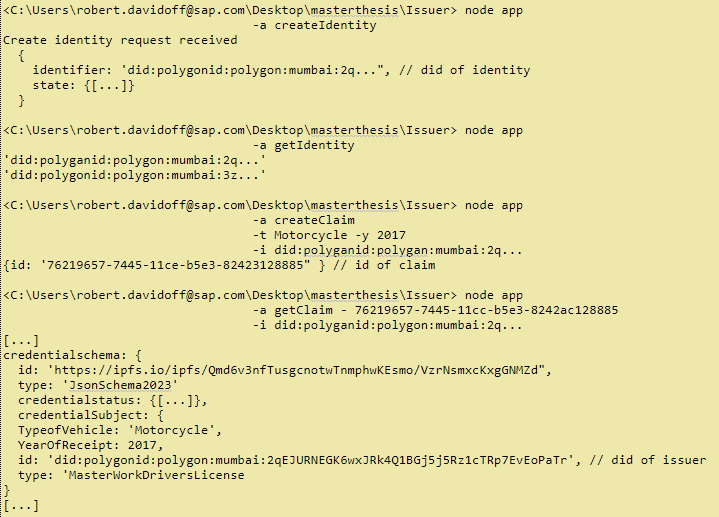
\includegraphics[scale=0.7]{media/CLI3}
		\caption{CLI Beispiele}
		\label{fig:CLI}
	\end{figure}
	
	Alle Implementierungen verwenden intern die REST-API des Issuer-Knoten. Alternativ zu ngrok ist es möglich dem Droplet eine 'reserved IP' zuzuweisen. Mittels PolygonScan (https://mumbai.polygonscan.com) und dem Monitoring Tool bei Alchemy sind die Aktivitäten auch als Transaktionen einsehbar. Nachdem der QR-Code gescannt wurde, kann man in der App den Credential einsehen, was in Abbildung \ref{fig:appCredential} ersichtlich wird.
	 \begin{figure}[H]
	 	\centering
	 	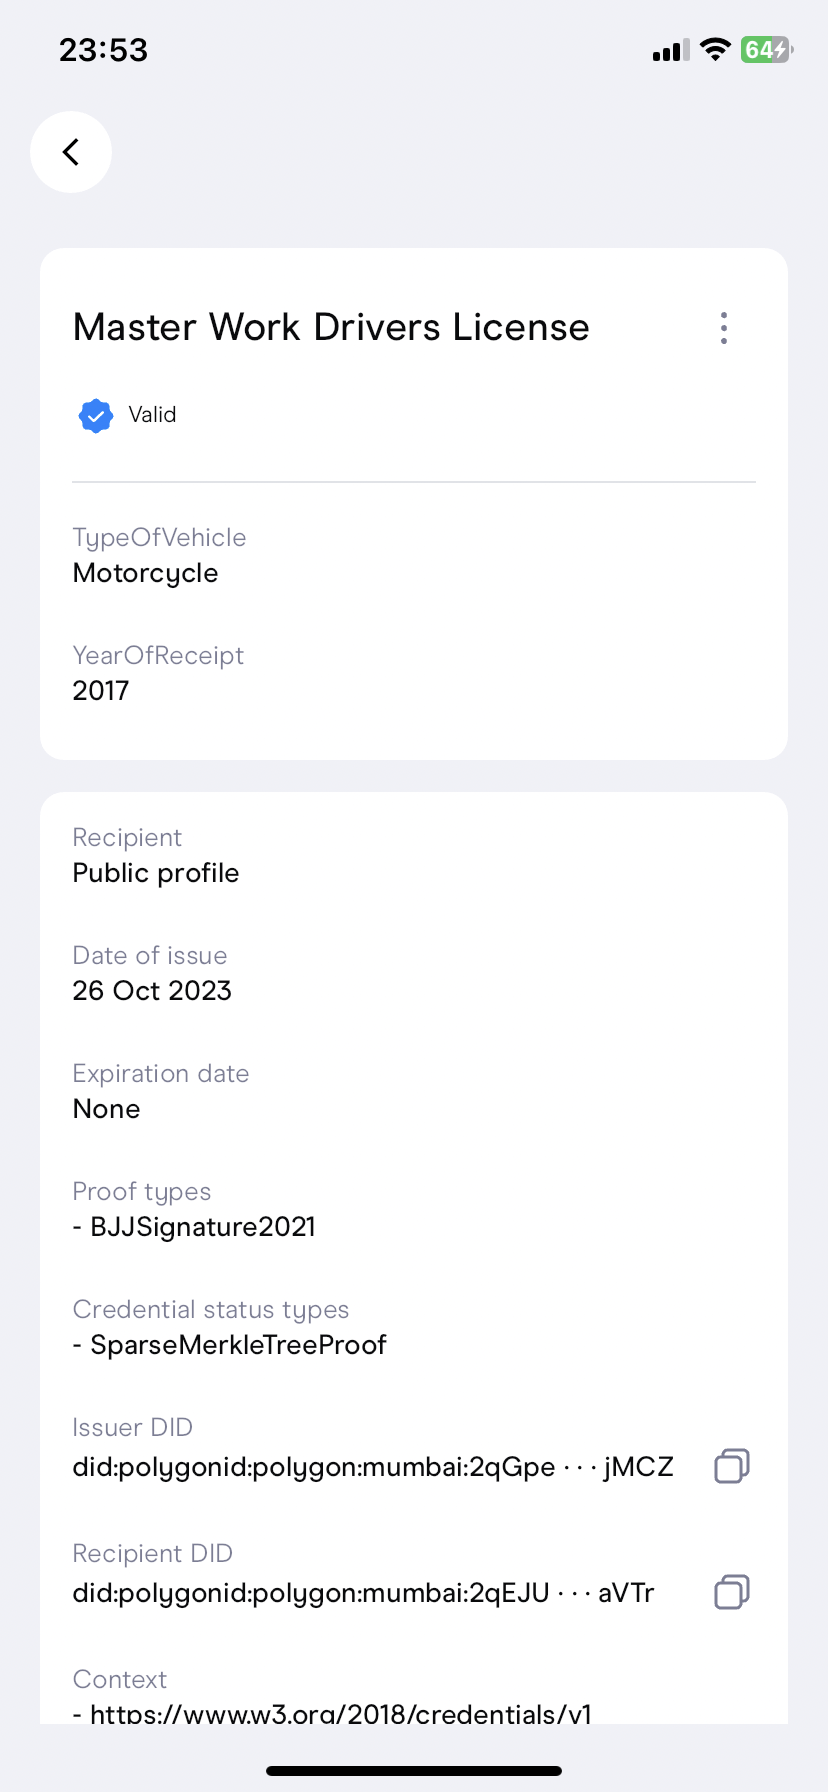
\includegraphics[scale=0.2]{media/appCredential}
	 	\caption{App Credential Beispiel}
	 	\label{fig:appCredential}
	 \end{figure}
	 
	 Es ist zu erkennen, dass die DID vom Issuer/Receiptient und die im CLI angegeben Attribute im Credential nachzuverfolgen sind.
	\end{itemize}
	 
\section{Der Verifier}
Der Verifier hat die Funktion die Credentials zu überprüfen. Hierbei wird zunächst überprüft, ob der Nutzer den Credential besitzt und ob er noch gültig ist, im Falle dass ein Auslaufdatum angegeben wurde oder der Credential widerrufen wurde. Drei Typen von Anfragen können gestellt werden:
\begin{itemize}
	\item Ohne Query: Entspricht einer Anfrage, die lediglich überprüft, ob der Credential existiert und valide ist
	\item Mit Query:
		\begin{itemize}
			\item Für Abfrage-Operatoren ungleich 'eq' (lt , gt, in, etc)
			\item Für Abfrage-Operation gleich 'eq'(entspricht ==). Dieser Typ von Anfragen wird auch als 'Selective Disclosure' bezeichnet.
		\end{itemize}
\end{itemize}
Gebaut werden können diese Anfragen mittels einem vom Polygon zur Verfügung gestellten Tool \cite{ID57}. Hierbei wird das Schema des Credentials geladen und über ein UI können die Attribute und Operatoren ausgewählt werden und ein JSON-Objekt wird als Ergebnis zurückgegeben.

Der oben beschriebe Query wird statisch im Programmcode festgehalten. \\
Über eine REST-API (gehostet auf port 8080) werden zwei Schnittstellen zur Verfügung gestellt:
\begin{itemize}
	\item /api: Dieser Endpunkt ist dafür zuständig den Request-Body zu bauen und zu speichern (wird später erneut benötigt). Zudem wird ein QRCode von dem Request abgespeichert, der mit der PolygonId-App gescannt werden kann. Der Request-Body sieht wie folgt aus:
	
\begin{lstlisting}[language=json,firstnumber=1]
{
	"from": "did:polygonid:polygon:mumbai:2qF57iujBWKeAGc2koCV56yW5S1SfPtFsCgDHzGRdW",
	"typ": "application/iden3comm-plain-json",
	"type": "https://iden3-communication.io/authorization/1.0/request",
	"body": {
		"reason": "Check if year of receipt is older than 2020",
		"callbackUrl": " https://df4c-165-1-191-123.ngrok-free.app/api/callback?sessionId=1",
		"scope": [
		{
			"id": 1,
			"circuitId": "credentialAtomicQuerySigV2",
			"query": {
				"allowedIssuers": ["*"],
				"type": "MasterWorkDriversLicense",
				"context": "https://ipfs.io/ipfs/QmTSd6saivXHysRopQdM1yswp2qyFwobL7fwuFpkVTS8gd",
				"credentialSubject": {
					"YearOfReceipt": {
						"$lt": 2020
					}
				}
			}
		}
		]
	}
}
\end{lstlisting}	
	\item /qr: Dient als Endpunkt, um die QR-Codes zu lesen
	\item /callback: Dieser Endpunkt von dem Identity-Wallet kontaktiert, um einen zk-Proof entgegenzunehmen und diesen zu verifizieren.
\end{itemize}
Nachdem der QR-Code von der App gescannt wurde, wird die Anfrage illustriert. Ebenso wird die URL des Issuers angezeigt und der Name des Credentials. Der Holder initiert die Verifizierung durch das Drücken des 'Approve'-Buttons. An dieser Stelle wird ein zk-Proof generiert und an den Verifier geschickt. Der Holder schickt hierfür einen POST-Request an die angegebene 'callbackURL'. An dieser Stelle führt der Server die tatsächliche Verifikation des zk-Proofs aus. Der Ablauf hierfür wird im folgenden Code beschrieben: \\ \\
\begin{lstlisting}[language = JavaScript , frame = trBL , firstnumber = last , escapeinside={(*@}{@*)}]
	const ethURL = 'https://polygon-mumbai.g.alchemy.com/v2/PRIVATE_API_KEY';
	const contractAddress = "0x134B1BE34911E39A8397ec6289782989729807a4" //public verification contract adress
	
	const ethStateResolver = new resolver.EthStateResolver(
	ethURL,
	contractAddress,
	);
	
	const resolvers = {
		['polygon:mumbai']: ethStateResolver,
	};
	
	
	// fetch authRequest from sessionID
	const authRequest = requestMap.get(`${sessionId}`);
	
	// EXECUTE VERIFICATION
	let path_full = path.join(__dirname, './circuits-dir')
	const verifier = await auth.Verifier.newVerifier(
	{
		stateResolver: resolvers,
		circuitsDir: path_full,
		ipfsGatewayURL:"https://app.pinata.cloud/gateway/amethyst-official-duck-350?pinataGatewayToken=F5FDkLi66xtMWFQ0BCjZ1EGceaWSvbQ1uvkioaYqi9Iq4lSc8CRpMi-2EXVSa1f" // gateway used to save the ZK-Proof
	}
);
\end{lstlisting}
Man kann erkennen, dass Pinata nicht nur verwendet um die Schemata zu speichern, sondern auch als Gateway, um die zk-Proofs abzulegen. Auch ist zu erkennen, dass eine URL für einen Polygon-Knoten notwendig ist, da zum einen auf Widerruf geprüft wird und zum anderen der unter 'contractAddress' gespeicherte Smart-Contract kontaktiert wird. Der Holder erhält im Anschluss die Information, dass mit Erfolg verifiziert wurde.

\subsection{On-Chain Verifikation}
An dieser Stelle sollte kurz erwähnt werden, dass es ebenso möglich wäre die Verifikation 'on-chain', also als Smart-Contract in der Blockchain ablaufen zu lassen. Hierbei wird - der in Solidity geschriebene - Smartcontract in der Blockchain deployed. Über einen Polygon-Knoten (beispielsweise gehostet über Alchemy) wird der - vom Holder erstelle - zk-Proof an den Smartcontract gesendet welcher die Richtigkeit überprüft. Der Vorteil hierbei wäre, dass der Gedanke der Dezentralität intensiviert wird und mehr Transparenz über die Verifikation gegeben wird. Als Nachteil ergibt sich, dass für das Deployment Vermögenswerte (MATIC) gezahlt werden müssen und Solidity weniger Schnittstellen bietet als Javascript.

\section{Der Holder}
Der Holder ist die Komponente mit der geringsten Relevanz für diesen . Es gibt jeweils eine App für Android und IOS, die folgende Funktionen haben \cite{ID58}:
\begin{itemize}
	\item SSI implementieren
	\item Credential entgegennehmen, speichern und warten
	\item zk-Proofs erstellen
	\item mit Issuer und Verifier kommunizieren
	\item Recovery-Funktion mittels 'seed-phrase'
\end{itemize}

Wenn ein Entwickler seinen eigenen 'Identity Wallet' implementieren möchte, hat er die Auswahl zwischen der Flutter-SDK (https://flutter.dev/) und einer Android SDK. Auch steht eine REST-API verschiedener Anbieter zur Verfügung, die Funktionen anbieten, die der Wallet benötigt, wie das Erstellen von Identitäten oder zk-Proofs.
Für diesen Prototypen wurde kein eigener Identity-Wallet implementiert, da der von Polygon-ID zur Verfügung gestellte Wallet bereits allen Anforderungen genügt und eine eigene Implementierung keinen Mehrwert liefert.

\section{Interaktion zwischen den Komponenten}
Um die Interaktion zwischen den Komponenten zu illustrieren wird folgende Grafik verwendet \ref{fig:trust}.

\begin{figure}[H]
	\centering
	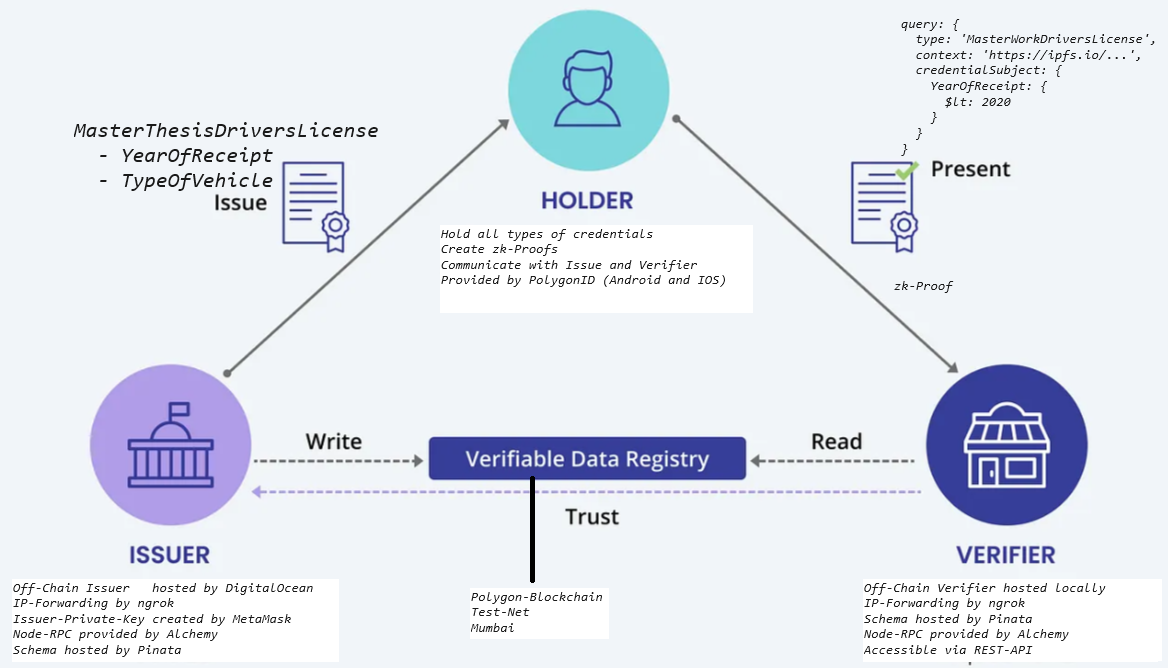
\includegraphics[scale=0.4]{media/trust}
	\caption{Interaktion zwischen den Komponenten \cite{ID63}}
	\label{fig:trust}
\end{figure}

Bei der Abbildung \ref{fig:trust} handelt es sich zunächst um das Konzept 'Triangle of Trust', dass mit den Details des Prototypen erweitert wurde. Unterhalb jeder der drei Komponenten werden technische Details zur Realisierung angegeben. Es ist zu erkennen, dass das Konzept abhängig davon ist, dass der Issuer korrekte Credentials angibt. In dem Szenario, dass der Issuer kompromittiert wurde oder bösartig ist würde folgende Situation eintreten:
\begin{itemize}
	\item Es werden fehlerhafte, unglaubwürdige Credential erstellt.
	\item Das Schreiben von Credentials in die Blockchain gilt als Transaktion und daher würden Kosten entstehen
	\item Der Holder ist im Besitzt dieser falschen Credentials und könnte (evtl. sogar unwissentlich Identitätsdiebstahl begehen)
	\item Der Verifier vertraut der 'Verifiable Data Registry' und würde fehlerhafte Credentials als richtig attestieren
\end{itemize} 
Daher ist die Korrektheit des Issuer von elementarer Bedeutung. \\
Ein schematischer Ablauf von der Erstellung der Identität des Issuer hin zur erfolgreichen Verifikation eines Credential des Holder sieht wie folgt aus \ref{fig:kommunikation}.
\begin{figure}[H]
	\centering
	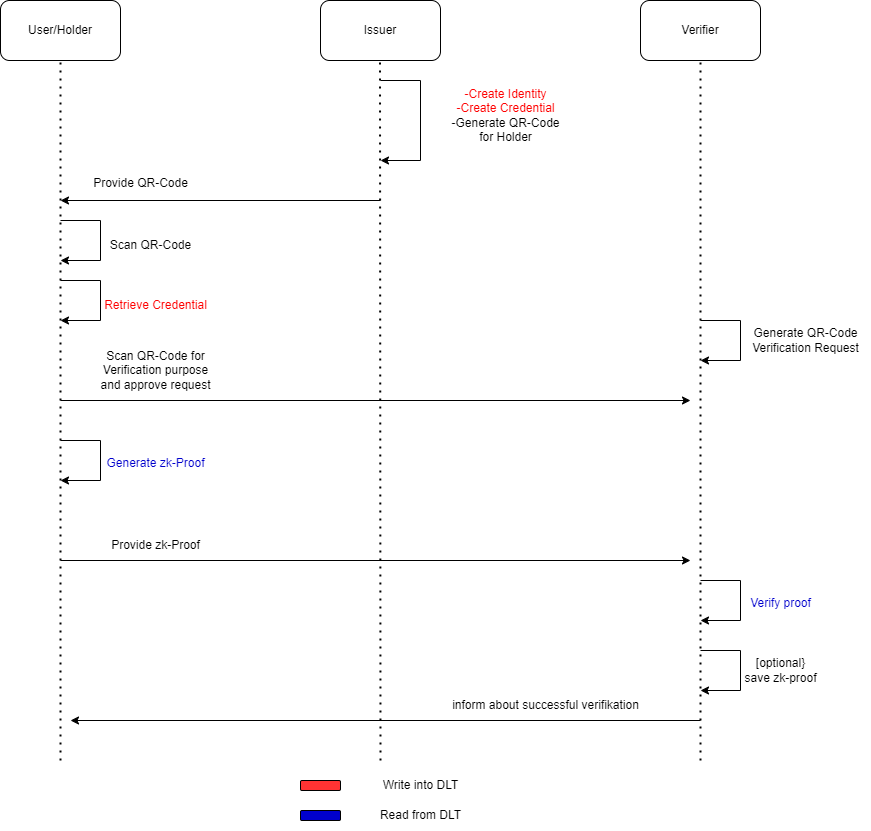
\includegraphics[scale=0.4]{media/kommunikation}
	\caption{Schematischer Ablauf des Prozesses}
	\label{fig:kommunikation}
\end{figure}
Rote Aktivitäten beinhalten Transaktionen in der Blockchain und blaue Aktivitäten beinhalten Leseprozesse. Außerdem ist zu sehen, dass viele Prozesse auf anderen Speichern arbeiten, wie z.B. verteile Speicher oder der lokale App-Speicher. Ein Unterschied zu Abbildung \ref{fig:komm} ist, dass der Verifier ebenso dargestellt ist und zwischen Lese- und Schreibzugriffen auf dem DLT unterschieden wird.
